\section{Introduction}
\label{s:DataGAIntroduction}
In this chapter, the generation of synthetic packet captures, together with the development and usage of the Jupyter analysis notebook, is elaborated.

The importance of automatically generating synthetic packet captures is stated in this chapter.
Having a standard of conducting each network scan enhances the reliability of each scan being conducted in a similar standardized way compared to manually running these Nmap scans, where differences might appear depending on the user inputs while executing the commands and human error.
In cases where this is conducted manually, the risk of not standardizing the scans can lead to incomparable data as an output during the analysis phase.
Therefore, the importance of automating the scans with a standard is crucial. The automation is also time-saving compared to a manual scanning procedure.
By the use of various timing templates, the workers finish the scans at different times, which makes a manual scanning method very time-consuming and not effective. This design and implementation chapter will describe the setup of such an automation packet capture generation.

A virtual lab environment was needed to conduct this research, with the purpose of segmenting captured scanning traffic from real internal network traffic to ensure the validity of the synthetic generated packet capture data, meanwhile having the capability of managing each worker host.
The importance of generating synthetic data is to have a clean data set, with minimal noise, for comparison against real-world data containing a substantial amount of noise traffic, as seen in figure \ref{fig:NoisePcap}.


\begin{figure}[htbp]
\centerline{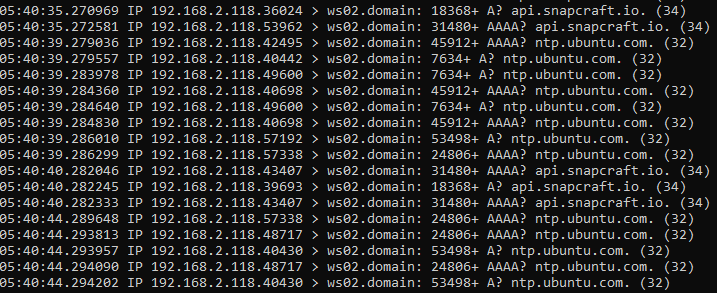
\includegraphics[scale=0.7]{images/misc/NoiseData.PNG}}
\caption{Capture of noise in packet capture.}
\label{fig:NoisePcap}
\end{figure}